\documentclass[a4paper]{IEEEtran}
\IEEEoverridecommandlockouts
% The preceding line is only needed to identify funding in the first footnote. If that is unneeded, please comment it out.
\usepackage{cite}
\usepackage{amsmath,amssymb,amsfonts}
\usepackage{algorithmic}
\usepackage{graphicx}
\usepackage{textcomp}
\usepackage{xcolor}
\usepackage{geometry}
\geometry{a4paper, portrait, margin=0.491in}

\def\BibTeX{{\rm B\kern-.05em{\sc i\kern-.025em b}\kern-.08em
    T\kern-.1667em\lower.7ex\hbox{E}\kern-.125emX}}
\begin{document}

\title{Bias in AI: Implementation Report \vspace{-0.2em}}

\author{\IEEEauthorblockN{Banner ID: 000810185 }\\ \textit{Dept. of Computer Science, Durham University}\vspace{-2em}}

\maketitle

\begin{abstract}
The following report details my implementation of a machine learning model that serves to mitigate algorithmic bias in sentiment analysis. The model follows an adversarial debiasing approach that neutralises underlying sentiment polarity in pre-trained word vectors for demographic identity terms.

The accompanying codebase has been thoroughly commented and carefully structured to ensure readability. Further information and insight regarding the project and specific implementation details can be found there.
\end{abstract}

\begin{IEEEkeywords}
algorithmic bias, machine learning, sentiment analysis, word embeddings, adversarial debiasing
\end{IEEEkeywords}

\section{Project Proposal}

\subsection{Background \& Motivation}

The bias that can be found in natural language processing (NLP) applications is a topic of personal intrigue. Generally, the various biases frequently observed within trained machine learning models can be traced back to the data that underscores these models. The altering of existing machine learning algorithms, or even the construction of entirely new ones, such that they mitigate bias is one remedy to this issue. Indeed, it's often the case that by improving the fairness of the original data collected and ultimately used by the models the biases would cease to arise in the first place. However, this is not a sustainable solution, sometimes due to various socio-economical or political factors that are beyond the control of whomever is responsible for the collection of the data, or even simply due to the general vagueness of ``fairness'', or how one can ensure a dataset is ``fair'' at all. I believe this principle applies to a substantial extent within the realm of NLP. 

Human language is inherently insufficient, thus it is brimming with bias. This fact facillitates a paritular issue with NLP programs, which will almost always rely on real-life instances of human discourse as their source of data. This could include news articles, reviews, actual conversations (e.g., message boards or social media), or even from human speech. The problem stemming from this is the difficulty in ensuring that the data is \textit{fair} - that is, that an even proportion of demographic groups are represented within the dialogue, that certain politically or idealogical sentiments aren't over-represented, or that the general chaotic nature of human discourse is accounted for. For these reasons, the acute importance of machine learning models with the capability of mitigating bias within the domain of NLP is highly apparent.

\subsection{Technical Details}

I intend to write a classifier for sentiment analysis, one that is initially biased, followed by one that has been ``debiased''. This will require a dataset containing sentences or phrases, labeled with an associated sentiment score.  Sentiment analysis is an application of natural language processing that I intuitively expect to be susceptible to bias as its primary concern is the emotive aspect of human language, which is steeped in subjectivity and, by extension, bias. Indeed, bias in sentiment analysis (and closely related tasks, such as toxicity detection) has been documented with respect to gender-, racial-, and age-related bias, each discussed in \cite{b1}, \cite{b2}, and \cite{b3}, respectively. 

A method of \textit{vectorising} the vocabulary to facilitate machine-interpretable text marks a further necessity. It is likely the case that the source of much of the bias will not only be derived from the sentence-sentiment dataset but from the word vectors used to represent the textual data. Thus, my primary concern with respect to \textit{debiasing} will pertain to the word vectors. % Based on my research, an adversarial machine learning approach appears suitable for a task such as this. 

The entire codebase will be written in Python as it is a language well suited for data analysis, machine learning, and NLP in particular. I intend to preprocess the sentence-sentiment dataset following traditional NLP methodology, using the NLTK Python library \cite{nltk}. The sentiment analysis will be created with a Support Vector Classifier, constructed using the scikit-learn library \cite{sklearn}. Finally, I anticipate the potential need of teaching myself a new machine learning framework in order to implement the adversarial debiasing model.

\section{Progress Report}

\subsection{The Data}

The dataset from the project suggestions that I have selected is the Stanford Sentiment Treebank (SST) dataset \cite{b4}. I was drawn to this dataset as it has been designed specifically for sentiment analysis tasks and contains several potential sources of bias. For instance, beside the inherent unpredictibility of human discourse and the bias embedded in language, the dataset itself is composed of sentences extracted from film reviews with sentiment scores labelled by human participants. These facts present two windows of potential bias, the latter in the biases that may be present in those labelling the sentences, and the former in terms of the biases associated with film reviewers. A report from the USC Annenberg Inclusion Initiative \cite{b5} detailed how the overwhelming majority of film reviewers are white and the prevailing gender is male. This lack of diversity implies that these sentences may not be representative of the discourse and vernacular of many demographics. % For instance, certain phrases may be more commonly used, which have varying interpretations amongst under-represented demographics. 

The bias-mitigation aspect of my implementation has been derived from \cite{b6}, which posits an in-processing adversarial debiasing model for mitigating underlying sentiment bias within word embeddings. %The article outlines an approach wherein a \textit{directional sentiment vector} is constructed from word embeddings, which can be used to project specific word vectors onto either a positive or negative sentiment subspace, thereby unveiling the underlying sentiment of this word - this plays a key role in the adversarial model, which primarily entails the detection of this underlying sentiment in demographic identity terms, and it's subsequent neutralisation.

To supplement the sentiment analysis and the process of debiasing, I have decided to utilise the \textit{word2vec} word embeddings (originally introduced by Google in 2013 \cite{b7}). These word embeddings are frequently used, especially for sentiment analysis and related NLP tasks, due to their effective capability of encapsulating semantics and word similarity. In particular, the embeddings that I will utilise will be pretrained on a large Google News corpus - demographic bias in relation to harmful cultural stereotypes in this specific version of the embeddings has actually been documented in \cite{b8}. 


%In addition to custom methods for detecting points of bias in the SST dataset and word embeddings,
I will utilise the Equity Evaluation Corpus (EEC) \cite{b9} to investigate the relative sentiment intensities predicted by the trained models, before and after debiasing, for sentences corresponding to the demographics of gender as well as race (European and African-American). As the EEC contains only these demographics, they will be the main demographics referenced during the project, without loss of generality. %As such, when this paper references ``Gender'', the ``Male'' and ``Female'' demographics are being referred to, and when ``Ethnicity'' is referenced, the ``African-American'' and ``European'' demographics are being referred to. %As the EEC only covers the two aforementioned ethnic demographics, I also intend to augment the dataset such that it is inclusive of other ethnic groups as well (e.g., Asian and Hispanic). 


\subsection{Data Analysis}

The original SST data is composed of several text files. The first functions in the codebase entail the downloading and configuring of these, whereby the sentiment analysis dataset is constructed. It comprises only two features, namely, ``sentences'' and ``sentiments''. The latter contains averages of many human-labeled sentiment scores corresponding with the former. Initially, these scores are continuous in the range $[0, 1]$, with smaller scores corresponding to more negative sentiment and vice versa. These scores are to be converted into binary in order to facilitate the binary classification problem, however this encoding is to be done at training time since the more verbose scores are convenient for data analysis, specifically with respect to bias.

The lack of explicit demographic labels within the data necessitated a manual procedure of searching for bias. My approach entailed utilising the EEC \cite{b9} to extract demographic identity terms pertaining to each gender and storing these in a list. These lists were augmented firstly with custom inputs followed by synonyms generated for each word in the lists, achieved using the NLTK library \cite{nltk}, specifically via the renowned \textit{wordnet} corpus \cite{wordnet}.  

The distributions of sentiment scores found for instances in the dataset wherein the sentence feature contains a word from one of the aforementioned lists is displayed in figure \ref{fig:sentiments-dist}. Although there is no clearly discernable bias in these distributions, it is noticeable that the Male sub-group is overrepresented compared to the Female sub-group, and likewise for European compared to African-American. This is reinforced by the data shown in table \ref{stats-table}, where little difference is apparent between the statistics other than the uneven sizes. These uneven proportions may be a potential source of bias.

\begin{figure}[htbp]
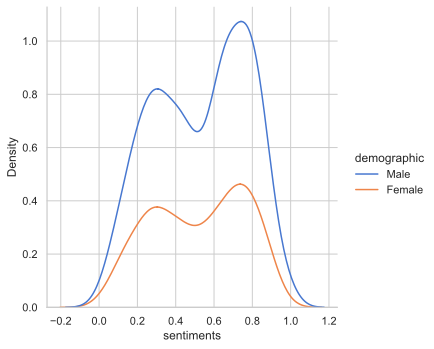
\includegraphics[width=0.48\linewidth]{images/male-female-sentiments.png}
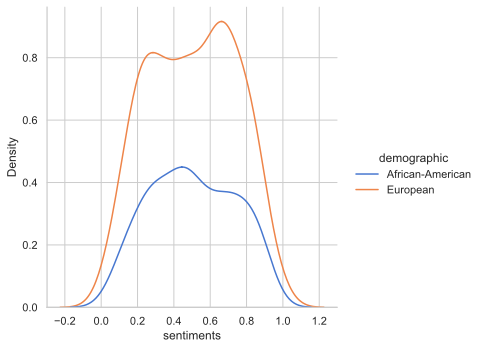
\includegraphics[width=0.48\linewidth]{images/aa-ee-sentiments.png}
\caption{Visualisations of the distribution of sentiments for the sentences containing words associated with the ``Male'' and ``Female'' demographic sub-groups (left) and the ``African-American'' and ``European'' sub-groups (right) in the Stanford Sentiment Treebank dataset.}
\label{fig:sentiments-dist}
\end{figure}

\begin{table}[htbp]
\caption{Stats. for Demographic Sub-groups in the SST Dataset}
\begin{center}
\begin{tabular}{|c|c|c|c|}
\hline
\multicolumn{2}{|c|}{\textbf{Demographic Sub-group}}&\multicolumn{2}{|c|}{\textbf{Sentiment Score Statistics}} \\
\cline{1-4} 
\textbf{Name} & \textbf{\textit{Size}}& \textbf{\textit{Mean}}& \textbf{\textit{Var.}} \\
\hline
Male & 1338 & 0.531 & 0.060 \\

Female & 592 & 0.518 & 0.059 \\
\hline
A.-A.$^{\mathrm{a}}$ & 158 & 0.503 & 0.053 \\

European & 336 & 0.502 & 0.058 \\

\hline
\multicolumn{4}{l}{$^{\mathrm{a}}$African-American.}
\end{tabular}
\label{stats-table}
\end{center}
\end{table}


To gain further intuition as to the presence of any bias, I produced \textit{wordclouds} for each demographic sub-group. Of note was the different results for the ethnicity demographics, shown in figure \ref{fig:clouds}. Here, certain words with negative connotations such as ``sinister'', ``bleak'', and ``grim'' were manifest in the African-American wordcloud, whereas equivalent patterns can not be found in the European wordcloud. This serves as an illustration of the subtle ways that bias may arise in NLP programs. 

\begin{figure}[htbp]
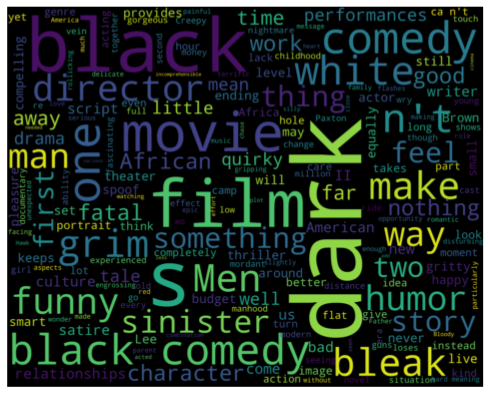
\includegraphics[width=0.48\linewidth]{images/aa-word-cloud-big.png}
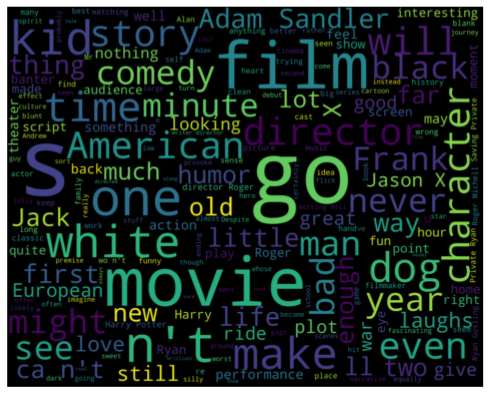
\includegraphics[width=0.48\linewidth]{images/e-word-cloud-big.png}
\caption{Wordclouds produced for sentences in the SST dataset containing vocabulary associated with the African-American (left) and European (right) demographic sub-groups.}
\label{fig:clouds}
\end{figure}

\subsection{Conventional Implementation}

The sentiment analysis was achieved via a Support Vector Classifier (SVC). The SST dataset was split into a training set comprising 75\% of the data and a testing set comprising the remaining 25\%. The preprocessing primarily included traditional NLP data tidying techniques derived from \cite{nltk}, which included conversion to lower case, stop word removal, lemmatisation, and word-tokenization. The vocabulary was vectorised with the word2vec embeddings \cite{b8}. The data was scaled via standard scaling and dimensionality reduction was incorporated via truncated singular value decomposition. 

The hyper-parameters, including the regularization parameter for the SVC, were optimised with cross-fold validation. This process was undertaken with care as, since the purpose of this project is to mitigate bias in sentiment analysis, it is crucial that any detected bias stems from more fundamental issues with NLP rather than a poorly configured model.

In terms of the model's performance, it achieved an overall accuracy score of 81\%, meaning it accuractely predicted 81\% of the sentiments in the testing data for the binary classification problem. Moreover, it attained an overall F1 score, precision score, and recall score also of 81\%. This indicates that the model successfully predicts the sentiments for both the positive and negative classes with minimal error. For more detail regarding the model performance, figure \ref{fig:variances} contains a ROC curve for each variant of the model trained. 

Despite the relative high performance of the model according to traditional metrics, bias was certainly present. Figure \ref{fig:sentiments} displays a the average sentiment score (in terms of probabilities) predicted by the model for sentences from the EEC corresponding to each demographic, relating to 5 different emotions. As the figure shows, there is a clear variance between the predictions for each demographic which indicates the presence of bias.

In order to gain further intuition as regards bias in the model, I constructed a simple sentiment analysis app. By inputting a sentence, a sentiment score is returned. A particular instance is displayed in figure \ref{fig:app}, which showcases that despite the two inputted sentences differing only in the demographic identity term used, one received a negative prediction whilst the other received a positive prediction, highlighting the effect that the biased model may have on a real-life downstream sentiment analysis application.

\begin{figure}[htbp]
\center{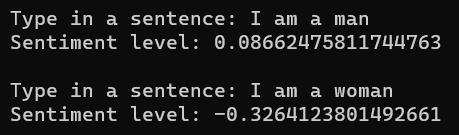
\includegraphics[width=0.6\linewidth]{images/app.png}}
\caption{Outcome of a simple sentiment analysis app utilising the classifer with no bias mitigation.}
\label{fig:app}
\end{figure}


\subsection{Unbiased Subsample}

Obtaining an unbiased subsample of the SST dataset was no trivial task due to the lack of demographic labels. To resolve this, I first implemented methods, akin to those described earlier with respect to the initial bias analysis, to append demographic labels to the dataset. Then, a logical approach was undertaken to ensure that the number of sentences associated with the female sub-group, where the corresponding binary sentiment score was positive, was equal to the number of sentences associated with the male demographic for positive sentiments. The same method was used to ensure equality in the negative sentiments also, and the same approach was taken for the ethnic demographic sub-groups (European and African-American). 

When the SVC was applied to this new subsampled dataset, the variance in EEC sentence predictions was reduced, as shown in figures \ref{fig:sentiments} and \ref{fig:variances}. However, there was a slight toll on the performance, with a marginally decreased accuracy score of 80\%. The minor decrease in overall performance is also illustrated in the ROC curve found in figure \ref{fig:sentiments}.

\subsection{Adversarial Debiasing}

\begin{figure}[htbp]
\centerline{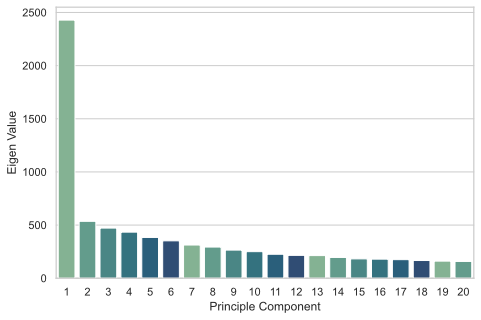
\includegraphics[width=0.4\linewidth]{images/pca-neg.png}
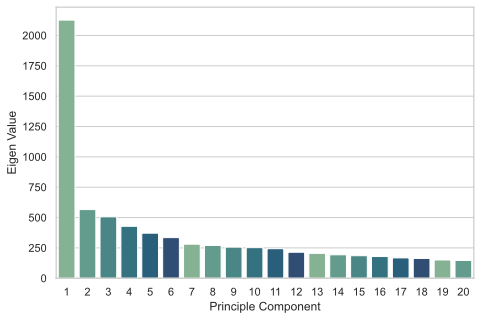
\includegraphics[width=0.4\linewidth]{images/pca-pos.png}}
\caption{The principle components of the negative (left) and positive (right) ground truth words vectors, used for the construction of the directional sentiment vector.}
\label{fig:pca}
\end{figure}

The theory underscoring my approach to debiasing the classifier is derived from \cite{b6}, which details an adversarial debiasing method for eradicating underlying sentiment bias in word embeddings. This first entailed the construction of a \textit{directional sentiment vector} (DSV), onto which word vectors can be projected in order to unveil their underlying sentiment polarity. To this end, the Opinion Lexicon dataset from \cite{lexicon} was used to obtain several thousand \textit{ground truth} positive and negative words, and the principle components obtained via PCA for corresponding positive and negative matrices comprising the word vectors for these ground truth words were obtained. The top 20 principle components for each are shown in figure \ref{fig:pca}. The signed difference between the most principle components of each composed the DSV, which had an accuracy of 91\%, closely matching the result from \cite{b6}. %By the methods outlined in \cite{b6} to measure the correctness of the DSV, I found it had an accuracy of 91\%.%, which closely match the results from \cite{b6}. %The signed difference between the most principle components of each composed the DSV. %By the methods outlined in \cite{b6} to measure the correctness of the DSV, I found it had an accuracy of 91\%.

As regards the adversarial debiasing algorithm, there is little instruction on practical implementations in the literature. Thus, I opted to implement the model purely from the available theory. I spent time to learn the machine learning framework PyTorch \cite{pytorch} as implementing it proved too difficult in pure Python. 

\begin{figure}[htbp]
\centerline{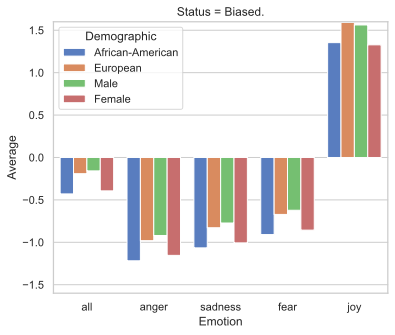
\includegraphics[width=0.44\linewidth]{images/before-debiasing.png}
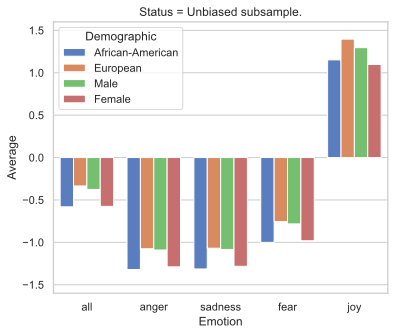
\includegraphics[width=0.44\linewidth]{images/subsample.png}}
\centerline{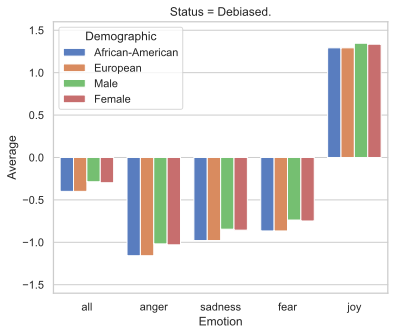
\includegraphics[width=0.44\linewidth]{images/after-debiasing.png}
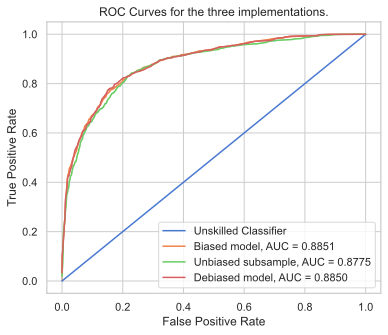
\includegraphics[width=0.44\linewidth]{images/roc.png}}
\caption{Sentiments predicted by the SVC trained with no bias-mitigating measures (top left), using the subsampled dataset (top right), and with the debiased embeddings (bottom left). A ROC curve is also included (bottom right) to showcase the relative performances of each implementation.}
\label{fig:sentiments}
\end{figure}

The algorithm serves to neutralise the sentiment polarity of demographic identity word vectors by minimising its projection onto the sentiment subspace whilst also evading semantic distortion. This is achieved via two competing loss functions - the \textit{predictor} loss function, that ensures the semantics represented by the word vector allign  with the original word vector, and the \textit{adversary} loss function, that describes the ability of an \textit{adversary} in predicting the sentiment polarity of the word vector being debiased. The algorithm aims to maximise the ability of the former whilst minimising that of the latter. 

Using PyTorch, I built a neural network utilising stochastic gradient descent to train the weights. The trained weights may be applied to word vectors within the embeddings to neutralise their sentiment polarity. Specifically, the weights are applied to many word vectors corresponding with demographic identity terms - the full list of these can be found in the codebase. Once applied, the original SVC is used to construct the sentiment analysis model. For more comprehensive discussion of the algorithm, consult the comments available in the codebase. 

This final implementation of the SVC attained an accuracy of 81\%. Together with the ROC curve from figure \ref{fig:sentiments}, this indicates the predictive ability of the sentiment analysis model has not been compromised by the debiasing. Figure \ref{fig:sentiments} showcases that the relative sentiment inensities assigned to the EEC sentences remains consistent, whilst the variance has been visibly reduced. As displayed in figure \ref{fig:variances}, the average variance amongst sentiment score predictions for sentences from the EEC is now $2.9\times10^{-3}$, which marks a significant reduction in disparity compared with the  conventional implementation using the subsampled dataset, where the variance was $1.2\times10^{-2}$. %(which itself was already a reduction from the variance of $6.5\times10^{-4}$ seen by the original, totally conventional implementation). 

\begin{figure}[htbp]
\centerline{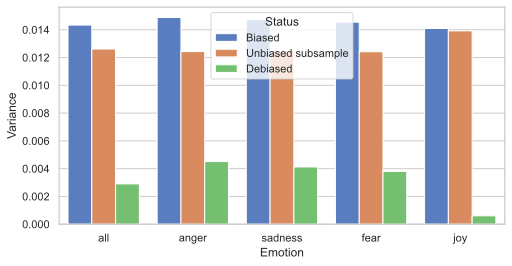
\includegraphics[width=0.85\linewidth]{images/variance-comparison.png}}
\caption{Comparison of the variances of the average sentiment scores for all demographics following each of the three approaches.}
\label{fig:variances}
\end{figure}

\section{Concluding Remarks}
%We can conlude that the primary source of sentiment bias in NLP tasks is the word embeddings used to represent the lexical data, and that the adversarial debiasing model posited in \cite{b6} is an effective strategy in the mitigation of such bias, as demonstrated by my implementation. 
There are certain limitations with the approach. Namely, the demographic identity terms must be specified by the developer as it is difficult to obtain an exhaustive list, so the model may facilitate unconscious bias in this respect. That said, this report illustrates that the adversarial algorithm is a complex, innovative, and effective contribution toward the reduction in bias present in NLP. In particular, it effectively reduces underlying sentiment bias in word embeddings, which can be very difficult to detect prior to usage in downstream applications. It has been shown that these debiased embeddings lead to a reduction in the bias present in a sentiment analysis model, with no compromise to the model's overall predictive performance.
%.. We can also discern that the model's predictive ability has not been compromised, because although the variability between the predictions for each demographic per emotion is reduced, the level of positivity or negativity is approximately the same as it was prior to applying the debiasing.
%As is observable for figure \ref{fig:sentiments}, the debiased model effectively reduces sentiment bias whilst maintaining the same levels of accuracy attained in the original, biased model. Moreover, it is clear that the adversarial learning approch is substanitally more successful than the subsample both in terms of the reduction in variance amongst the EEC predictions, but also in terms of model performance. This confirms my initial predictions that the word embeddings would have a significantly greater impact on the bias contained within sentiment analysis programs compared to the sentence-sentiment dataset used.



%\section{Concluding Remarks}

%Although the model has been shown to effectively eradicate underlying sentiment bias contained within word vectors, whilst simultaneously maintaining a reasonable degree of semantic similarity with the original embeddings, the model itself does have several limitations. Perhaps the most significant is that the potentially biased vocabulary must be specified by the developer, as the model doesn't detect them independently. The issue here is derived from the fact that an exhaustive list of demographic terminology is exceedingly difficult to attain, especially due to language's ever-shifting nature. Furthermore, this dependence may facilitate bias, intentional or not, on the developer's end. 


\newpage

\begin{thebibliography}{00}
\bibitem{b1} M. Thelwall. (2018, Feb.). Gender bias in sentiment analysis. \textit{Online Information Review} [Online]. 42(1), pp. 45-57. Available: https://doi.org/10.1108/OIR-05-2017-0139 
\bibitem{b2} M. Sap, D. Card, S. Gabriel, Y. Choi, N. A. Smith. ``The risk of racial bias in hate speech detection,'' in \textit{Proc. 57th Annu. Meeting of the Association for Computational Linguistics}, Stroudsburg, PA, USA, 2019, pp. 1668–1678.
\bibitem{b3} M. Diaz, I. Johnson, A. Lazar, A. M. Piper, D. Gergle. ``Addressing age-related bias in sentiment analysis,'' in \textit{2018 Proc. Conf. Human Factors in Computing Systems}, New York, NY, USA, pp. 1-14.
\bibitem{nltk} S. Bird, E. Loper, E. Klein. (2010, Jan.). Natural Language Processing with Python. [Online]. Available: https://www.nltk.org/book/
\bibitem{sklearn} F. Pedregosa, G. Varoquaux, A. Gramfort, V. Michel, B. Thirion, O. Grisel, et al. (2011). Scikit-learn: machine learning in python. \textit{J. Machine Learning Research} [Online]. 12(85), pp. 2825-2830. Available: https://jmlr.csail.mit.edu/papers/v12/pedregosa11a.html
\bibitem{b4} R. Socher, A, Perelygin, J. Y. Wu, J. Chuang, C. D. Manning, A. Y. Ng, C. Potts. ``Recursive deep models for semantic compositionality over a sentiment treebank,'' in \textit{Proc. 2013 Conf. Empirical Methods in Natural Language Processing}, Seattle, WA, USA, pp. 1631-1642. SST dataset available: https://nlp.stanford.edu/sentiment/code.html
\bibitem{b5} M. Choueiti, S. L. Smith, K. Pieper, A. Chase. (2018, Sep.). Critic's Choice 2: Gender and Race/Ethnicity of Film Reviewers Across 300 Top Films from 2015-2017. Annenberg Inclusion Initiative, CA. [Online]. Available: http://assets.uscannenberg.org/docs/cricits-choice-2018.pdf
\bibitem{b6} C. Sweeney, M. Najafian. ``Reducing sentiment polarity for demographic attributes in word embeddings using adversarial learning,'' In \textit{Proc. 2020 Conf. Fairness, Accountability, and Transparency (FAT* '20)}, New York, NY, USA, pp. 359–368.
\bibitem{b7} T. Mikolov, G. S. Corrado, K. Chen, J. Dean. ``Efficient estimation of word representations in vector space,'' in \textit{Int. Conf. Learning Representations}, Scottsdale, AR, USA, 2013, pp. 1-12. Embeddings available: https://code.google.com/archive/p/word2vec/ 
\bibitem{b8} N. Garg, L. Schiebinger, D. Jurafsky, J. Zou, ``Word embeddings quantify 100 years of gender and ethnic stereotypes," \textit{Proc. Nat. Academy of Sciences}, vol. 115, issue 16, April 2018. 
\bibitem{b9} S. Kiritchenko, S. M. Mohammad. ``Examining gender and race bias in two hundred sentiment analysis systems,'' in \textit{Proc. 7th Joint Conf.  Lexical and Computational Semantics (*SEM)}, New Orleans, LA, USA, 2018. EEC dataset available: https://saifmohammad.com/WebPages/Biases-SA.html
\bibitem{lexicon} M. Hu, B. Liu. ``Mining and summarizing customer reviews,'' in \textit{Proc. 10th ACM SIGKDD Int. Conf. Knowledge Discovery and Data Mining}, New York, NY, USA, 2004, pp. 168–177. Opinion lexicon dataset available: https://www.cs.uic.edu/~liub/FBS/sentiment-analysis.html
\bibitem{wordnet} \textit{About WordNet}, Princeton University, Princeton, NJ, 2010. Available: https://wordnet.princeton.edu/
\bibitem{pytorch} A. Paszke, S. Gross, F. Massa, A. Lerer, J. Bradbury, G. Chanan, et al. ``Pytorch: an imperative style, high-performance deep learning library,'' in \textit{Advances in Neural Information Processing Systems 32}, Vancouver, BC, Canada, 2019, pp. 8024-8035.
\end{thebibliography}


\end{document}
